\documentclass[11pt]{article}
\usepackage[margin=18mm,headheight=22pt]{geometry}
\usepackage{amsmath}
\usepackage{fontspec}
\usepackage{unicode-math}
\setmainfont{NewCM10}[Extension=.otf,UprightFont=*-Book,BoldFont=*-Bold,ItalicFont=*-BookItalic,BoldItalicFont=*-BoldItalic]
\setsansfont{NewCMSans10}[Extension=.otf,UprightFont=*-Book,BoldFont=*-Bold,ItalicFont=*-BookOblique,BoldItalicFont=*-BoldOblique]
\setmathfont{NewCMMath-Book.otf}
\usepackage{xcolor}
\definecolor{FAUblue}{HTML}{04316A}
\definecolor{Paperblue}{HTML}{EEF2F7}
\definecolor{EEIgold}{HTML}{CC9C42}
\usepackage{etoolbox,enumitem,booktabs,tabularx,array,needspace,microtype}
\usepackage[most]{tcolorbox}
\usepackage{titlesec,fancyhdr}
\usepackage[hidelinks]{hyperref}
\usepackage{draftwatermark}
\SetWatermarkText{Made by Thanate Amornjiraporn (Focus)}
\SetWatermarkColor{black!7}\SetWatermarkFontSize{30pt}\SetWatermarkAngle{45}
\setlength{\parindent}{0pt}
\setlength{\parskip}{5pt}
\setlist{itemsep=2pt,topsep=3pt,leftmargin=1.6em,beginpenalty=10000,endpenalty=10000}
\raggedbottom
\clubpenalty=10000 \widowpenalty=10000 \displaywidowpenalty=10000 \interlinepenalty=10000
\setcounter{secnumdepth}{0}
\setcounter{tocdepth}{1}
\pagestyle{fancy}\fancyhf{}
\fancyhead[L]{\small\sffamily\color{FAUblue} From Fundamentals to AI Apocalypse · EEI · Tutorial 6}
\fancyhead[R]{\small\sffamily Tutorial 6: Worked solutions}
\fancyfoot[C]{\small\thepage}
\titleformat{\section}{\Large\bfseries\sffamily\color{FAUblue}}{}{0pt}{}
\titleformat{\subsection}{\large\bfseries\sffamily\color{FAUblue}}{}{0pt}{}
\titlespacing*{\section}{0pt}{16pt}{6pt}
\preto\section{\Needspace{8\baselineskip}}
\preto\subsection{\Needspace{6\baselineskip}}
\newtcolorbox{equationcard}[1]{colback=Paperblue,colframe=Paperblue,boxrule=0pt,arc=0pt,left=10pt,right=10pt,top=6pt,bottom=6pt,title={#1},fonttitle=\small\bfseries\sffamily,coltitle=FAUblue,before skip=8pt,after skip=8pt}
\newtcolorbox{workedbox}[1]{colback=white,colframe=EEIgold,boxrule=0pt,leftrule=3pt,arc=0pt,left=10pt,top=4pt,bottom=4pt,title={#1},fonttitle=\small\bfseries\sffamily,coltitle=FAUblue,attach title to upper={\par},before skip=8pt,after skip=8pt}
\newtcolorbox{recallbox}[1]{colback=white,colframe=FAUblue,boxrule=0pt,leftrule=3pt,arc=0pt,left=10pt,top=4pt,bottom=4pt,title={#1},fonttitle=\small\bfseries\sffamily,coltitle=FAUblue,attach title to upper={\par},before skip=8pt,after skip=8pt}
\usepackage{environ}
\newsavebox\measurebox
% Typeset the section once invisibly to measure it; start a new page if it will not fit in what is left.
\makeatletter
\newif\ifkeep@measuring
\NewEnviron{keepsection}{%
  \ifkeep@measuring \BODY \else
    \edef\keep@sec{\the\value{section}}\edef\keep@sub{\the\value{subsection}}%
    \setbox\measurebox\vbox{\hsize\linewidth\keep@measuringtrue\def\Needspace##1{}\BODY}%
    \setcounter{section}{\keep@sec}\setcounter{subsection}{\keep@sub}%
    \dimen2=\ht\measurebox \advance\dimen2\dp\measurebox
    \dimen@=\textheight
    \ifdim\pagegoal<\maxdimen
      \dimen@=\pagegoal \advance\dimen@-\pagetotal
      \ifdim\dimen2>\dimen@ \clearpage \dimen@=\textheight \fi
    \fi
    % if it fits, nothing inside may force an early break
    \ifdim\dimen2>\dimen@ \BODY \else \begingroup\def\Needspace##1{}\BODY\endgroup \fi
  \fi}
\makeatother
\newtcolorbox{notebox}{colback=Paperblue,colframe=Paperblue,boxrule=0pt,arc=0pt,left=8pt,right=8pt,top=4pt,bottom=4pt,before skip=6pt,after skip=6pt}
\newtcolorbox{plainbox}{colback=white,colframe=FAUblue,boxrule=0pt,leftrule=3pt,arc=0pt,left=10pt,right=8pt,top=4pt,bottom=4pt,before skip=6pt,after skip=8pt}
\usetikzlibrary{arrows.meta}
\title{\sffamily\bfseries\color{FAUblue}Tutorial 6: Worked solutions}
\author{Electrical Engineering I \ensuremath{\cdot} Module 92315 \ensuremath{\cdot} Tutorial 6\\[2pt]\small From Fundamentals to AI Apocalypse · personal study guide}
\date{}
\begin{document}
\maketitle
\begingroup\footnotesize\setlength{\parskip}{0pt}\tableofcontents\endgroup
\clearpage

\Needspace{8\baselineskip}
{\large Track the conserved current through each cylindrical sector, use local Ohm’s law in each material, then integrate the radial field across both layers.}


\begin{keepsection}
\Needspace{11\baselineskip}
\section{Task 10: Stationary electric flow field}

\Needspace{8\baselineskip}
The conductor is an annular sector with axial height \textit{h} and angular span α. An ideal inner electrode at radius \textit{a}\textsubscript{0} feeds current through material κ\textsubscript{1} from \textit{a}\textsubscript{0} to \textit{a}\textsubscript{1}, then through material κ\textsubscript{2} from \textit{a}\textsubscript{1} to \textit{a}\textsubscript{2} to the outer electrode. Take positive \textit{I} and \textit{U}\textsubscript{12} in the outward direction from electrode 1 to electrode 2, as drawn; use α in radians.

\Needspace{9\baselineskip}
\textbf{Connected topic:} Current density (§2.1.2) and local Ohm’s law (§2.2.2) determine the radial fields; resistance (§2.2.4) follows by integrating through the layered path.

\Needspace{14\baselineskip}
\begin{center}
\begin{minipage}[t]{0.950\linewidth}\centering
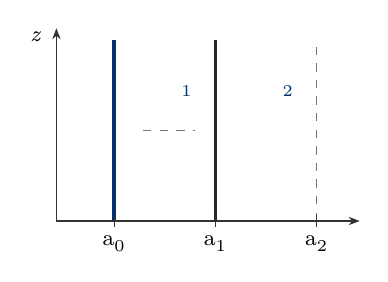
\begin{tikzpicture}[line join=round]
\draw[-{Stealth[length=4pt]},black!80] (0.720,-2.628) -- (4.572,-2.628);
\draw[-{Stealth[length=4pt]},black!80] (0.720,-2.628) -- (0.720,-0.180);
\draw[FAUblue,line width=1.6pt] (1.454,-2.628) -- (1.454,-0.324);
\draw[black!85,line width=1pt] (2.740,-2.628) -- (2.740,-0.324);
\draw[black!55,dashed] (4.025,-2.628) -- (4.025,-0.324);
\draw[black!55,dashed] (1.822,-1.476) -- (2.483,-1.476);
\node[anchor=west,text=FAUblue,inner sep=1pt,font=\footnotesize] at (2.187,-0.976) {κ\textsubscript{1}};
\node[anchor=west,text=FAUblue,inner sep=1pt,font=\footnotesize] at (3.472,-0.976) {κ\textsubscript{2}};
\node[anchor=east,inner sep=1pt,font=\footnotesize] at (4.536,-2.916) {\textit{ρ}};
\node[anchor=east,inner sep=1pt,font=\footnotesize] at (0.576,-0.288) {\textit{z}};
\draw[black!80] (1.454,-2.556) -- (1.454,-2.700);
\node[,inner sep=1pt,font=\footnotesize] at (1.454,-2.916) {a\textsubscript{0}};
\draw[black!80] (2.740,-2.556) -- (2.740,-2.700);
\node[,inner sep=1pt,font=\footnotesize] at (2.740,-2.916) {a\textsubscript{1}};
\draw[black!80] (4.025,-2.556) -- (4.025,-2.700);
\node[,inner sep=1pt,font=\footnotesize] at (4.025,-2.916) {a\textsubscript{2}};
\end{tikzpicture}\par\smallskip{\small\raggedright \textbf{Meridian view of the radial current path.} The cross-section is revolved through angle α; at radius ρ, the current passes through area α ρ h. The interface at \textit{a}\textsubscript{1} separates the two conductivities.\par}\end{minipage}
\end{center}

\begin{keepsection}
\Needspace{7\baselineskip}
\subsection{10a: Set up the current-density field}

\Needspace{4\baselineskip}
Try first: use charge conservation at steady state and the normal-current boundary condition at the κ\textsubscript{1}/κ\textsubscript{2} interface.

\nopagebreak[4]{\small\itshape Answers: see “Task 10: Stationary electric flow field” under Answers at the end.}
\end{keepsection}

\begin{keepsection}
\Needspace{7\baselineskip}
\subsection{10b: Find \textit{J} as a function of \textit{I}}

\Needspace{4\baselineskip}
Try first: calculate the area normal to radial flow at radius ρ, then divide the total current by that area.

\nopagebreak[4]{\small\itshape Answers: see “Task 10: Stationary electric flow field” under Answers at the end.}
\end{keepsection}

\begin{keepsection}
\Needspace{6\baselineskip}
\subsection{10c: Find the electric field strength}

\Needspace{3\baselineskip}
Try first: apply \textit{J} = κ\textit{E} separately in each radial layer.

\nopagebreak[4]{\small\itshape Answers: see “Task 10: Stationary electric flow field” under Answers at the end.}
\end{keepsection}

\begin{keepsection}
\Needspace{7\baselineskip}
\subsection{10d: Find \textit{U}\textsubscript{12}(\textit{I})}

\Needspace{4\baselineskip}
Try first: integrate the radial field along the current path, changing conductivity at the material boundary.

\nopagebreak[4]{\small\itshape Answers: see “Task 10: Stationary electric flow field” under Answers at the end.}
\end{keepsection}

\begin{keepsection}
\Needspace{7\baselineskip}
\subsection{10e: Find the resistance}

\Needspace{4\baselineskip}
Try first: divide the voltage from 10d by the current, or add the two layer resistances in series.

\nopagebreak[4]{\small\itshape Answers: see “Task 10: Stationary electric flow field” under Answers at the end.}
\end{keepsection}
\end{keepsection}


\clearpage
\section{Answers}
\begin{keepsection}\subsection{Task 10: Stationary electric flow field}

\begin{workedbox}{10a \ensuremath{\cdot} Continuity across the layers}
\Needspace{11\baselineskip}
\begin{enumerate}
\item In a stationary flow, charge does not accumulate in the conductor, so the net current through each coaxial sector surface is the same. At the interface ρ = \textit{a}\textsubscript{1}, the normal is \textit{e}\textsubscript{ρ}: its normal current component is continuous, and the tangential electric-field components (zero here) are continuous too.
\item \Needspace{5\baselineskip}
The current flows radially, normal to the cylindrical interface. Therefore \textit{J}\textsubscript{ρ,1} = \textit{J}\textsubscript{ρ,2}. Local Ohm’s law \textit{J} = κ\textit{E} means the electric field generally changes at the interface:

\begin{equation*}{E}_{ρ,2}/{E}_{ρ,1}\, =\, κ_{1}/κ_{2}\end{equation*}
\item The ideal electrodes have κ \ensuremath{\to} \ensuremath{\infty}, so their internal electric field is zero while they remain equipotential. Neglect edge spreading at the ends of the sector; the current in the two finite-conductivity layers is radial.
\end{enumerate}
\end{workedbox}

\end{keepsection}
\begin{keepsection}\subsection{Task 10: Stationary electric flow field}

\begin{workedbox}{10b \ensuremath{\cdot} Current through a cylindrical sector}
\Needspace{7\baselineskip}
\begin{enumerate}
\item \Needspace{5\baselineskip}
At radius ρ, the curved surface spans arc length α ρ and axial height \textit{h}, so its area normal to the flow is:

\begin{equation*}{A}({ρ})\, =\, α\, {ρ\,h}\end{equation*}
\item \Needspace{5\baselineskip}
By symmetry the radial current density is uniform over this surface, and \textit{I} = $\int $ \textit{J} \ensuremath{\cdot} d\textit{A} = \textit{J}\textsubscript{ρ}\textit{A}(\textit{ρ}):

\Needspace{5\baselineskip}
\begin{equation*}{J}({ρ})\, =\, [{I}/(α\, {h\,ρ})]{e}_{ρ},\, \quad \, {a}_{0}\, <\, {ρ}\, <\, {a}_{2}\end{equation*}

The same expression holds on both sides of \textit{a}\textsubscript{1}. It falls as 1/ρ because the current-carrying area grows with radius.
\end{enumerate}
\end{workedbox}

\end{keepsection}
\begin{keepsection}\subsection{Task 10: Stationary electric flow field}

\begin{workedbox}{10c \ensuremath{\cdot} Piecewise Ohm’s law}
\Needspace{6\baselineskip}
\begin{enumerate}
\item \Needspace{4\baselineskip}
In the first layer, \textit{a}\textsubscript{0} \ensuremath{<} ρ \ensuremath{<} \textit{a}\textsubscript{1}, divide the current density by κ\textsubscript{1}:

\begin{equation*}{E}_{1}({ρ})\, =\, [{I}/(α\, {h\,κ}_{1}{ρ})]{e}_{ρ}\end{equation*}
\item \Needspace{4\baselineskip}
In the second layer, \textit{a}\textsubscript{1} \ensuremath{<} ρ \ensuremath{<} \textit{a}\textsubscript{2}, use κ\textsubscript{2} instead:

\Needspace{5\baselineskip}
\begin{equation*}{E}_{2}({ρ})\, =\, [{I}/(α\, {h\,κ}_{2}{ρ})]{e}_{ρ}\end{equation*}

At the interface the normal current remains continuous, while \textit{E} jumps by the conductivity ratio found in 10a. The direction is outward for positive \textit{I}.
\end{enumerate}
\end{workedbox}

\end{keepsection}
\begin{keepsection}\subsection{Task 10: Stationary electric flow field}

\begin{workedbox}{10d \ensuremath{\cdot} Voltage drop across both layers}
\Needspace{8\baselineskip}
\begin{enumerate}
\item \Needspace{5\baselineskip}
With \textit{U}\textsubscript{12} defined as electrode-1 potential minus electrode-2 potential, it equals the outward field integral from \textit{a}\textsubscript{0} to \textit{a}\textsubscript{2}. Split the integral where κ changes:

\begin{equation*}{U}_{12}\, =\, \int_{{a}_{0}}^{{a}_{1}} \, {E}_{1,ρ}\, \mathrm{d}{ρ}\, +\, \int_{{a}_{1}}^{{a}_{2}} \, {E}_{2,ρ}\, \mathrm{d}{ρ}\end{equation*}
\item \Needspace{4\baselineskip}
Substitute the fields and integrate dρ/ρ in each interval:

\Needspace{4\baselineskip}
\begin{equation*}{U}_{12}({I})\, =\, [{I}/(α\, {h\,κ}_{1})]\, \ln ({a}_{1}/{a}_{0})\, +\, [{I}/(α\, {h\,κ}_{2})]\, \ln ({a}_{2}/{a}_{1})\end{equation*}

The voltage is positive for outward positive current. Each logarithm is dimensionless.
\end{enumerate}
\end{workedbox}

\end{keepsection}
\begin{keepsection}\subsection{Task 10: Stationary electric flow field}

\begin{workedbox}{10e \ensuremath{\cdot} Series resistance of radial layers}
\Needspace{7\baselineskip}
\begin{enumerate}
\item \Needspace{5\baselineskip}
Resistance is \textit{R} = \textit{U}\textsubscript{12}/\textit{I}. Since the current passes through κ\textsubscript{1} and κ\textsubscript{2} sequentially, their radial resistances add:

\begin{equation*}{R}_{1}\, =\, \ln ({a}_{1}/{a}_{0})/(α\, {h\,κ}_{1}),\, \quad \, {R}_{2}\, =\, \ln ({a}_{2}/{a}_{1})/(α\, {h\,κ}_{2})\end{equation*}
\item \Needspace{4\baselineskip}
Therefore:

\Needspace{5\baselineskip}
\begin{equation*}{R}\, =\, 1/(α\, {h})[\ln ({a}_{1}/{a}_{0})/κ_{1}\, +\, \ln ({a}_{2}/{a}_{1})/κ_{2}]\end{equation*}

The units are ohms: 1/(κh) has units Ω, and the angle and logarithms are dimensionless. If κ\textsubscript{1} = κ\textsubscript{2} = κ, the logs combine to ln(\textit{a}\textsubscript{2}/\textit{a}\textsubscript{0}), a useful check.
\end{enumerate}
\end{workedbox}

\end{keepsection}

\vfill{\small Personal worked-solution guide based on the supplied EE1 Tutorial Task sheet, written in my own words; no tutorial text or figures are reproduced. Not an official FAU publication; check course details against current material. Made by \textbf{Thanate Amornjiraporn (Focus)}.}

\end{document}
